% Options for packages loaded elsewhere
\PassOptionsToPackage{unicode}{hyperref}
\PassOptionsToPackage{hyphens}{url}
\documentclass[
]{ltjsarticle}
\usepackage{xcolor}
\usepackage[margin=2.5cm]{geometry}
\usepackage{amsmath,amssymb}
\setcounter{secnumdepth}{-\maxdimen} % remove section numbering
\usepackage{iftex}
\ifPDFTeX
  \usepackage[T1]{fontenc}
  \usepackage[utf8]{inputenc}
  \usepackage{textcomp} % provide euro and other symbols
\else % if luatex or xetex
  \usepackage{unicode-math} % this also loads fontspec
  \defaultfontfeatures{Scale=MatchLowercase}
  \defaultfontfeatures[\rmfamily]{Ligatures=TeX,Scale=1}
\fi
\usepackage{lmodern}
\ifPDFTeX\else
  % xetex/luatex font selection
\fi
% Use upquote if available, for straight quotes in verbatim environments
\IfFileExists{upquote.sty}{\usepackage{upquote}}{}
\IfFileExists{microtype.sty}{% use microtype if available
  \usepackage[]{microtype}
  \UseMicrotypeSet[protrusion]{basicmath} % disable protrusion for tt fonts
}{}
\makeatletter
\@ifundefined{KOMAClassName}{% if non-KOMA class
  \IfFileExists{parskip.sty}{%
    \usepackage{parskip}
  }{% else
    \setlength{\parindent}{0pt}
    \setlength{\parskip}{6pt plus 2pt minus 1pt}}
}{% if KOMA class
  \KOMAoptions{parskip=half}}
\makeatother
\usepackage{graphicx}
\makeatletter
\newsavebox\pandoc@box
\newcommand*\pandocbounded[1]{% scales image to fit in text height/width
  \sbox\pandoc@box{#1}%
  \Gscale@div\@tempa{\textheight}{\dimexpr\ht\pandoc@box+\dp\pandoc@box\relax}%
  \Gscale@div\@tempb{\linewidth}{\wd\pandoc@box}%
  \ifdim\@tempb\p@<\@tempa\p@\let\@tempa\@tempb\fi% select the smaller of both
  \ifdim\@tempa\p@<\p@\scalebox{\@tempa}{\usebox\pandoc@box}%
  \else\usebox{\pandoc@box}%
  \fi%
}
% Set default figure placement to htbp
\def\fps@figure{htbp}
\makeatother
\setlength{\emergencystretch}{3em} % prevent overfull lines
\providecommand{\tightlist}{%
  \setlength{\itemsep}{0pt}\setlength{\parskip}{0pt}}
\usepackage[haranoaji]{luatexja-preset}
\usepackage{bookmark}
\IfFileExists{xurl.sty}{\usepackage{xurl}}{} % add URL line breaks if available
\urlstyle{same}
\hypersetup{
  hidelinks,
  pdfcreator={LaTeX via pandoc}}

\author{}
\date{}

\begin{document}

\section{位置揺らぎを持つ光源による二重スリット干渉の思考実験 ―
光源位置分布の縞シフト量分布への押し出し（形の保存）}\label{ux4f4dux7f6eux63faux3089ux304eux3092ux6301ux3064ux5149ux6e90ux306bux3088ux308bux4e8cux91cdux30b9ux30eaux30c3ux30c8ux5e72ux6e09ux306eux601dux8003ux5b9fux9a13-ux5149ux6e90ux4f4dux7f6eux5206ux5e03ux306eux7e1eux30b7ux30d5ux30c8ux91cfux5206ux5e03ux3078ux306eux62bcux3057ux51faux3057ux5f62ux306eux4fddux5b58}

\textbf{木原 範昭}

\emph{本稿は\textbf{思考実験（モデル計算）}であり、実測ではない。確立した物理（標準的な波動光学・量子力学）を覆す主張は一切含まない。特定の幾何配置のもとで、光源位置の確率分布が、反復試行における遠方場干渉縞のシフト量の確率分布へどのように写されるかを、厳密な解析・数値計算によって例示するものである。}

バージョン v0.3（2026-06-29） DOI (Version): 10.5281/zenodo.21035809 DOI
(Concept): 10.5281/zenodo.21035808 Zenodo:
https://zenodo.org/records/21035809

\begin{center}\rule{0.5\linewidth}{0.5pt}\end{center}

\subsection{要旨}\label{ux8981ux65e8}

静止した点光源が、その位置に波長の半分 \(\pm\lambda/2\)
のオーダの揺らぎを持つと仮定し、二重スリットを通した遠方場の干渉を考える。光源位置
\(y\)
が与えられた一回の試行では、干渉縞は\textbf{同じ形のまま、純粋な幾何学的経路差だけ左右にシフト}した一枚の縞として現れる（波長は全域で
\(\lambda_0\) 一定、振動数偏移は関与しない）。縞中央ピークのシフト量
\(u(y)\) は、光源位置の\textbf{ほぼ線形な写像}である。

本稿の主張はこれである。\textbf{光源位置 \(y\) を確率分布 \(P(y)\)
に従って試行ごとにランダムに引く反復観測において、各試行の縞シフト量
\(u\) の確率分布は \(P\)
の押し出し（pushforward）\(\rho(u)=P(y(u))\,|dy/du|\) であり、写像
\(u(y)\) が線形であるため、\(P\)
がどんな形であってもその形が保存される。}
これは新しい確率法則の導出ではなく、入力分布が（ほぼ線形な幾何写像を通じて）シフト量の分布へ写される変数変換（押し出し）の例示である。本稿では
\(P(y)=\cos^2(\pi y/\lambda)\) を具体例として用い、シフト量分布が同形の
\(\cos^2\) になることを示す。形からの \(\sim2\text{–}3\%\)
のずれは、写像 \(u(y)\) の非近軸的な非線形性（非近軸スケール
\(\tfrac12\tan^2\theta\approx3\%\)）に由来し、近軸極限 \(W/L\to0\)
で消失する。

重要な但し書きとして、この分布は\textbf{一回の観測像の属性ではない}。一回の試行は一つのシフト量（一枚の縞）を与えるだけである。また、多数試行の強度を一枚のスクリーンに\textbf{積算}した像は、シフトで畳み込まれた\textbf{可視度の低下した単一縞}であって、入力分布の形にはならない。形が現れるのは、各試行でシフト量を読み、それを反復してヒストグラムを作るときである（光源位置が試行内で準静的、試行間で揺らぐことを仮定する）。

\begin{center}\rule{0.5\linewidth}{0.5pt}\end{center}

\subsection{1. はじめに}\label{ux306fux3058ux3081ux306b}

二重スリット干渉は、波動光学と量子力学の双方で基本的な思考実験の舞台である。本稿では、光源位置に揺らぎがあるとき、反復観測において縞のシフト量にどのような統計が現れるかを問う。

結論を先取りすれば、各試行は同じ縞をシフトさせるだけであり、シフト量は光源位置のほぼ線形な写像である。したがって、光源位置を分布
\(P(y)\) から反復してランダムに引けば、\textbf{シフト量の分布は \(P\)
の押し出しとして、近軸で同形を保つ}。これは新しい確率法則の導出ではなく、入力分布が観測される統計量（シフト量）へ写される変数変換の例示である。\(P(y)=\cos^2(\pi y/\lambda)\)
を例にとり、シフト量分布が同形の \(\cos^2\) となること、ずれが非近軸
\(\tfrac12\tan^2\theta\approx3\%\)
にとどまることを示す。本稿は思考実験であり、すべては指定した幾何配置の上での厳密計算である。

\begin{center}\rule{0.5\linewidth}{0.5pt}\end{center}

\subsection{2. 実験条件}\label{ux5b9fux9a13ux6761ux4ef6}

\subsubsection{2.1 全体配置}\label{ux5168ux4f53ux914dux7f6e}

単一の点光源 \(S\)（波長 \(\lambda_0=1\), 光速 \(c=1\)）が、距離
\(L=10\) にある二重スリットを照らす。スリット間隔は
\(W=5\)、スリットは光軸に対し上下対称（\(y=\pm W/2=\pm2.5\)）に置く。各スリットは光源から見て光軸に対し半角
\(\theta=\arctan(0.25)\approx14.04^\circ\)
をなす。スクリーンは遠方（\(D\gg L\)、フラウンホーファー領域）にあるとする。

\begin{figure}
\centering
\pandocbounded{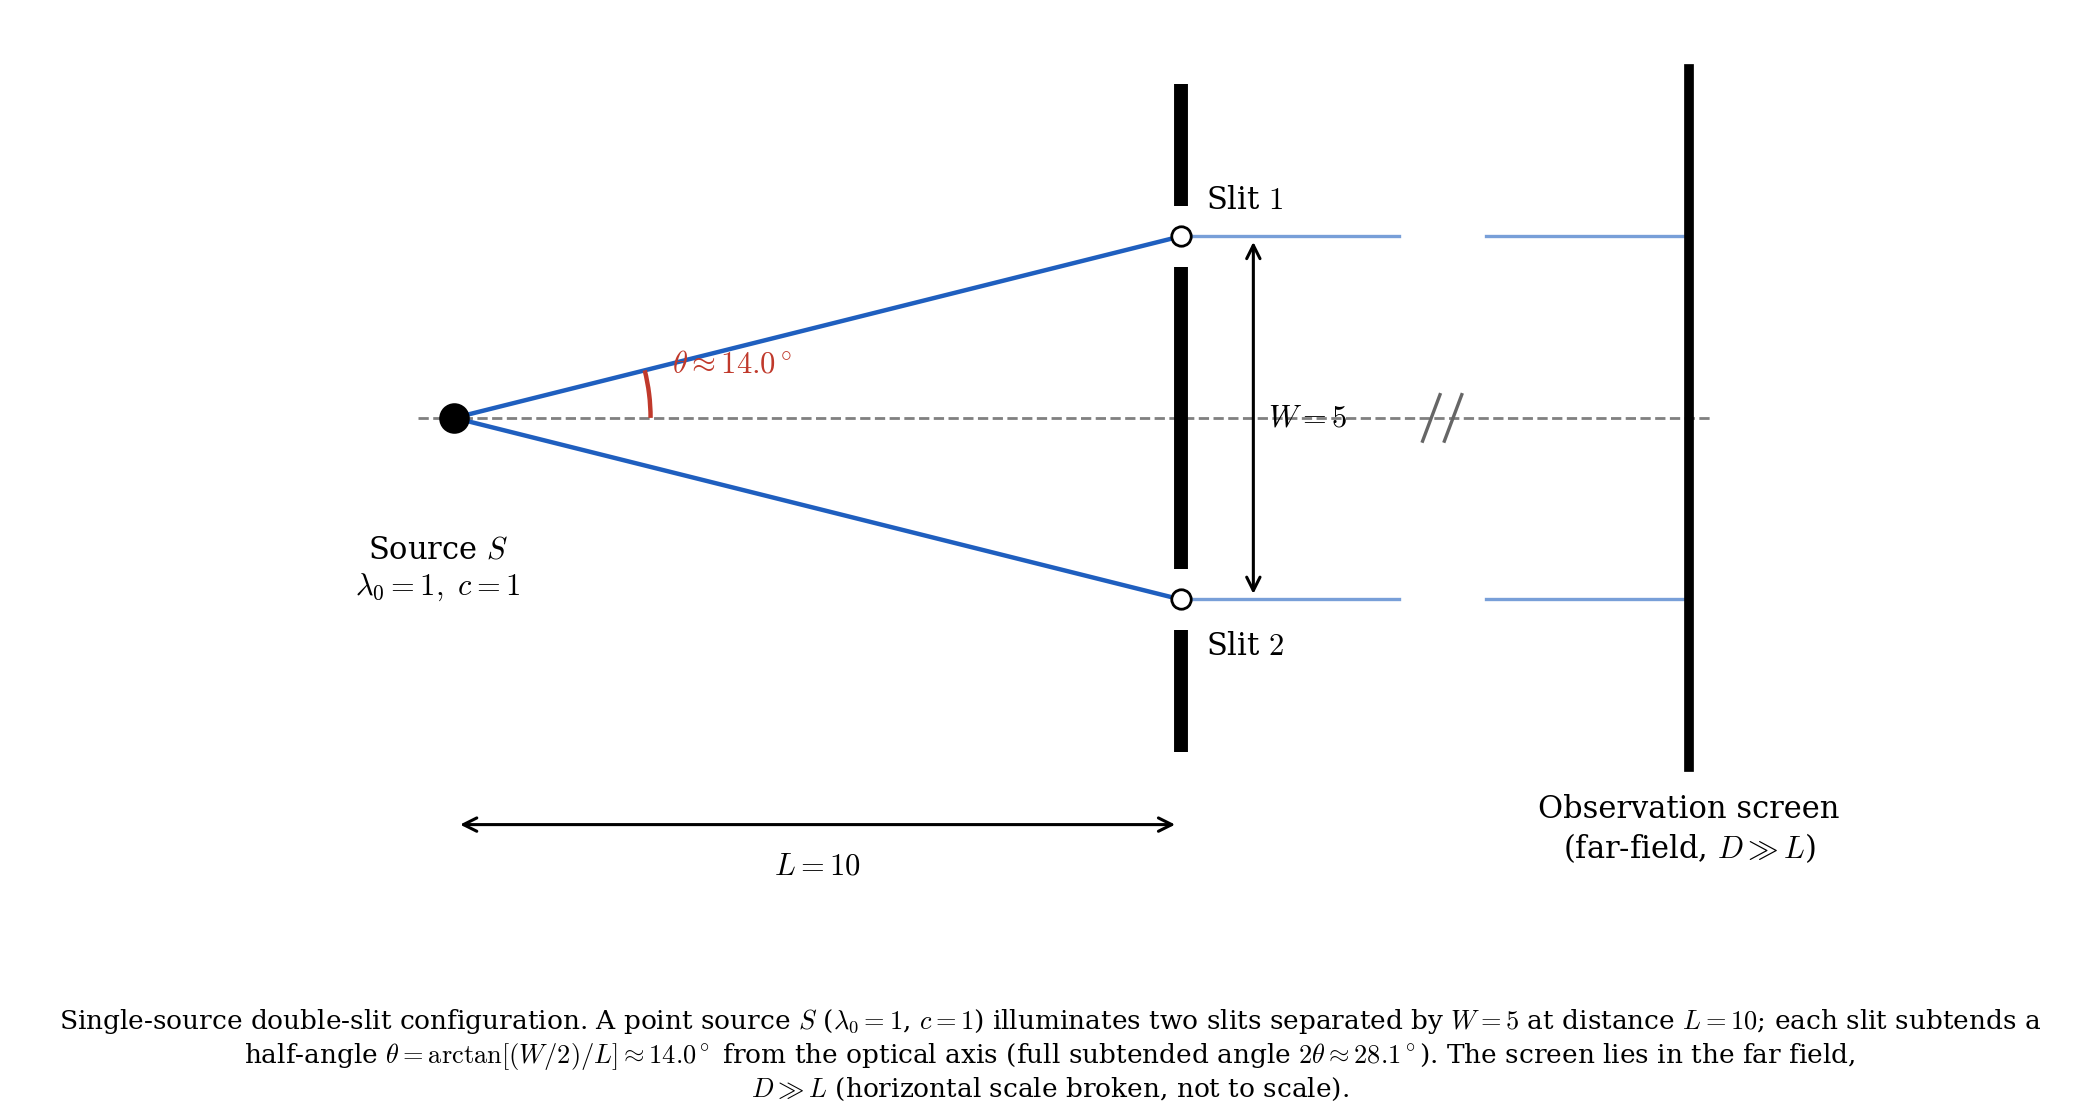
\includegraphics[keepaspectratio,alt={図1 全体配置}]{fig_setup_double_slit.png}}
\caption{図1 全体配置}
\end{figure}

\emph{図1：単一光源・二重スリットの全体配置（\(L=10\), \(W=5\),
\(\lambda_0=1\), \(c=1\)）。各スリットは光軸から半角
\(\theta\approx14^\circ\)。スクリーンは遠方（横方向は破断・非スケール）。}

\subsubsection{2.2
光源位置の揺らぎ}\label{ux5149ux6e90ux4f4dux7f6eux306eux63faux3089ux304e}

光源位置に半径 \(\lambda/2\)
の不確定性を与え、スクリーンに平行な（横方向の）位置 \(y\)
の確率分布を、具体例として

\[P(y)=\cos^2\!\Big(\frac{\pi y}{\lambda}\Big),\qquad y\in[-\tfrac{\lambda}{2},\,\tfrac{\lambda}{2}]\]

と置く（中央でピーク、\(\pm\lambda/2\)
でゼロの中央ピーク型釣鐘）。本稿では位置スケールの \(\lambda\)
と光の波長 \(\lambda_0\)
を同一にとる（\(\lambda=\lambda_0=1\)）。この分布を入力とし、その由来は問わない。光源位置は\textbf{1試行内では準静的に固定され、試行間でこの
\(P(y)\) に従ってランダムに引き直される}とする。

\begin{figure}
\centering
\pandocbounded{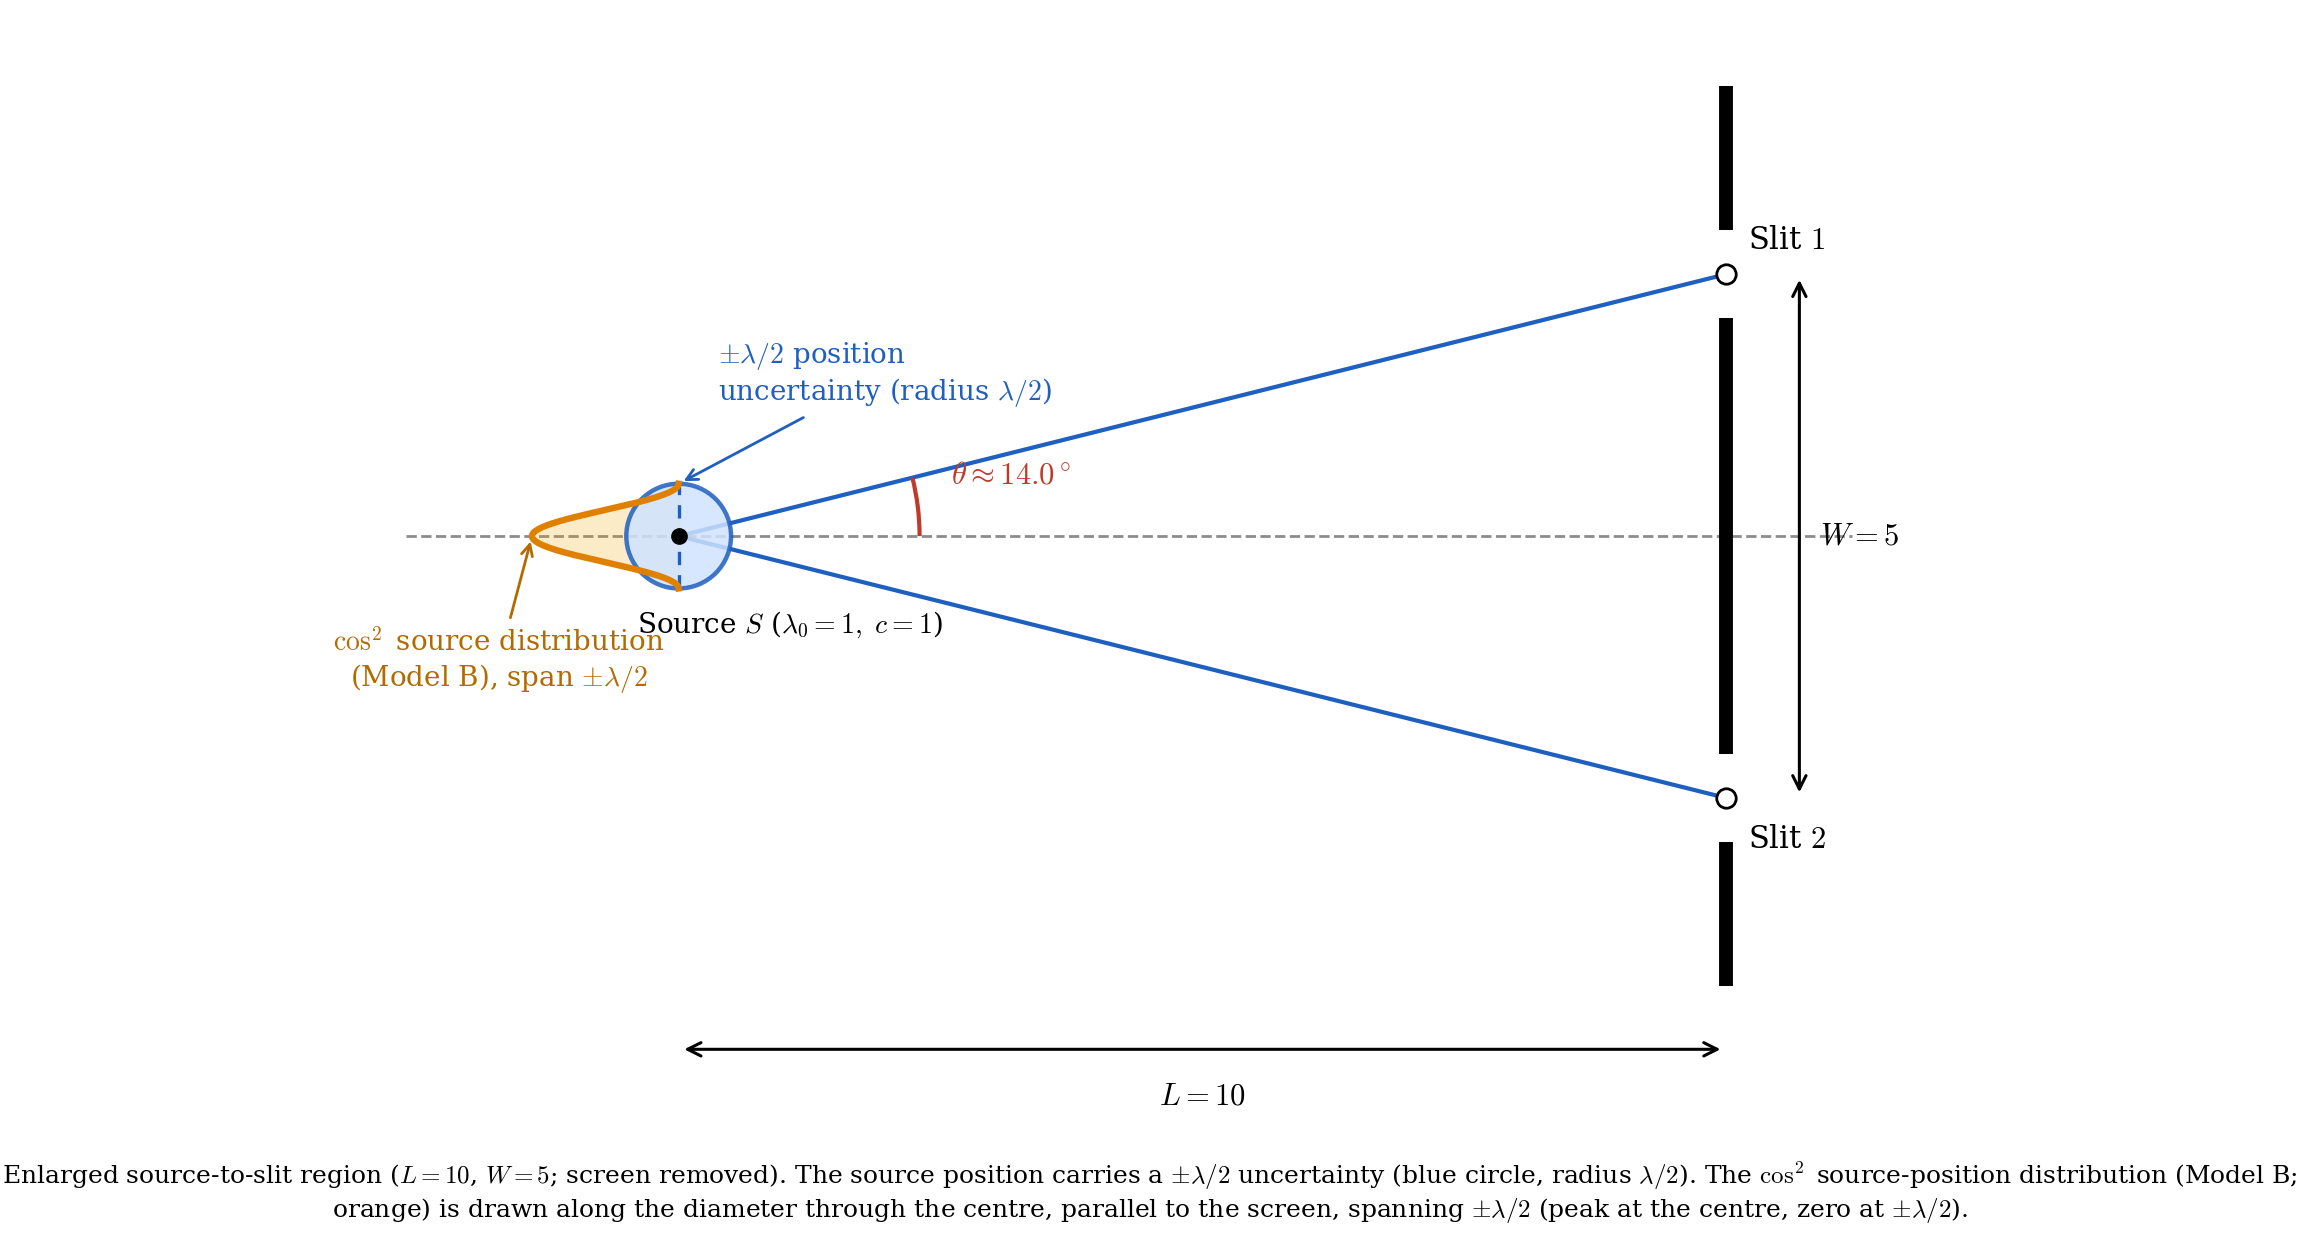
\includegraphics[keepaspectratio,alt={図2 光源位置の揺らぎ}]{fig_setup_source_uncertainty.png}}
\caption{図2 光源位置の揺らぎ}
\end{figure}

\emph{図2：光源〜スリット領域の拡大図（\(L=10\),
\(W=5\)、スクリーンは削除）。光源位置は半径 \(\lambda/2\)
の不確定円（青）を持ち、中心を通りスクリーンに平行な軸に沿って
\(P(y)=\cos^2\)
分布（橙、\(\pm\lambda/2\)、中央ピーク・端ゼロ）が乗る。}

\begin{center}\rule{0.5\linewidth}{0.5pt}\end{center}

\subsection{3.
方法（純幾何モデル）}\label{ux65b9ux6cd5ux7d14ux5e7eux4f55ux30e2ux30c7ux30eb}

光源 \(S=(-L,\,y)\)、スリット \(A_1=(0,+W/2)\)、\(A_2=(0,-W/2)\)
とする。スクリーン点を遠方場の回折角
\(\theta_s\)（\(s=\sin\theta_s\)）で表す。波長は全域で \(\lambda_0\)
一定とする（移動仮定もドップラーも導入しない。光は静止光源から \(c\)
で伝播するが、放射点が動かない以上、振動数偏移は生じない）。

各アーム \(k\)
の位相は、光源側の幾何学的経路と遠方場のスクリーン側経路差の和で与えられる：

\[\Phi_k(s;y)=\frac{2\pi}{\lambda_0}\Big[\,r_k(y)-y_{{\rm slit},k}\,s\,\Big],\qquad
r_k(y)=\sqrt{L^2+(y-y_{{\rm slit},k})^2}.\]

干渉強度（複素共役による厳密なボルン形式）は

\[I(s;y)=\big|e^{i\Phi_1}+e^{i\Phi_2}\big|^2
=2+2\cos\!\Big[\tfrac{2\pi}{\lambda_0}\big(\Delta r(y)-W s\big)\Big],\qquad \Delta r(y)=r_1-r_2.\]

\(y\) に依るのは位相オフセット \(\Delta r(y)\)
だけで、\textbf{波形は厳密に同形}（「同形のままシフト」は近似ではなく厳密）。縞中央ピーク（\(\Delta\Phi=0\)）の位置は

\[u(y)\equiv\Phi_0^{\rm peak}(y)=\frac{2\pi}{\lambda_0}\,\Delta r(y)\ \approx\ -\frac{2\pi W}{L\lambda_0}\,y\quad(\text{近軸で線形})\]

で与えられる（横軸はスリット基準位相 \(\Phi_0=2\pi W s/\lambda_0\)）。

\begin{center}\rule{0.5\linewidth}{0.5pt}\end{center}

\subsection{4. 結果}\label{ux7d50ux679c}

\subsubsection{4.1
シフト量分布＝押し出し}\label{ux30b7ux30d5ux30c8ux91cfux5206ux5e03ux62bcux3057ux51faux3057}

各光源位置の干渉を別々に描くと、各試行は同形の縞を \(u(y)\)
だけシフトさせる（図3）。シフト量 \(u\) の確率分布は \(P\) の押し出し

\[\rho(u)=P\big(y(u)\big)\,\Big|\frac{dy}{du}\Big|\]

である。\(u(y)\) が線形なら \(|dy/du|\) は定数で、\textbf{\(\rho(u)\) は
\(P\) と同形になる（軸が伸縮するだけ）。これは \(\cos^2\)
固有の性質ではなく、線形写像が任意の入力 \(P\)
の形を保つことの帰結である。} 本稿の例 \(P=\cos^2(\pi y/\lambda)\) では
\(\rho(u)\propto\cos^2(\pi u/180^\circ)\) となる。

\begin{figure}
\centering
\pandocbounded{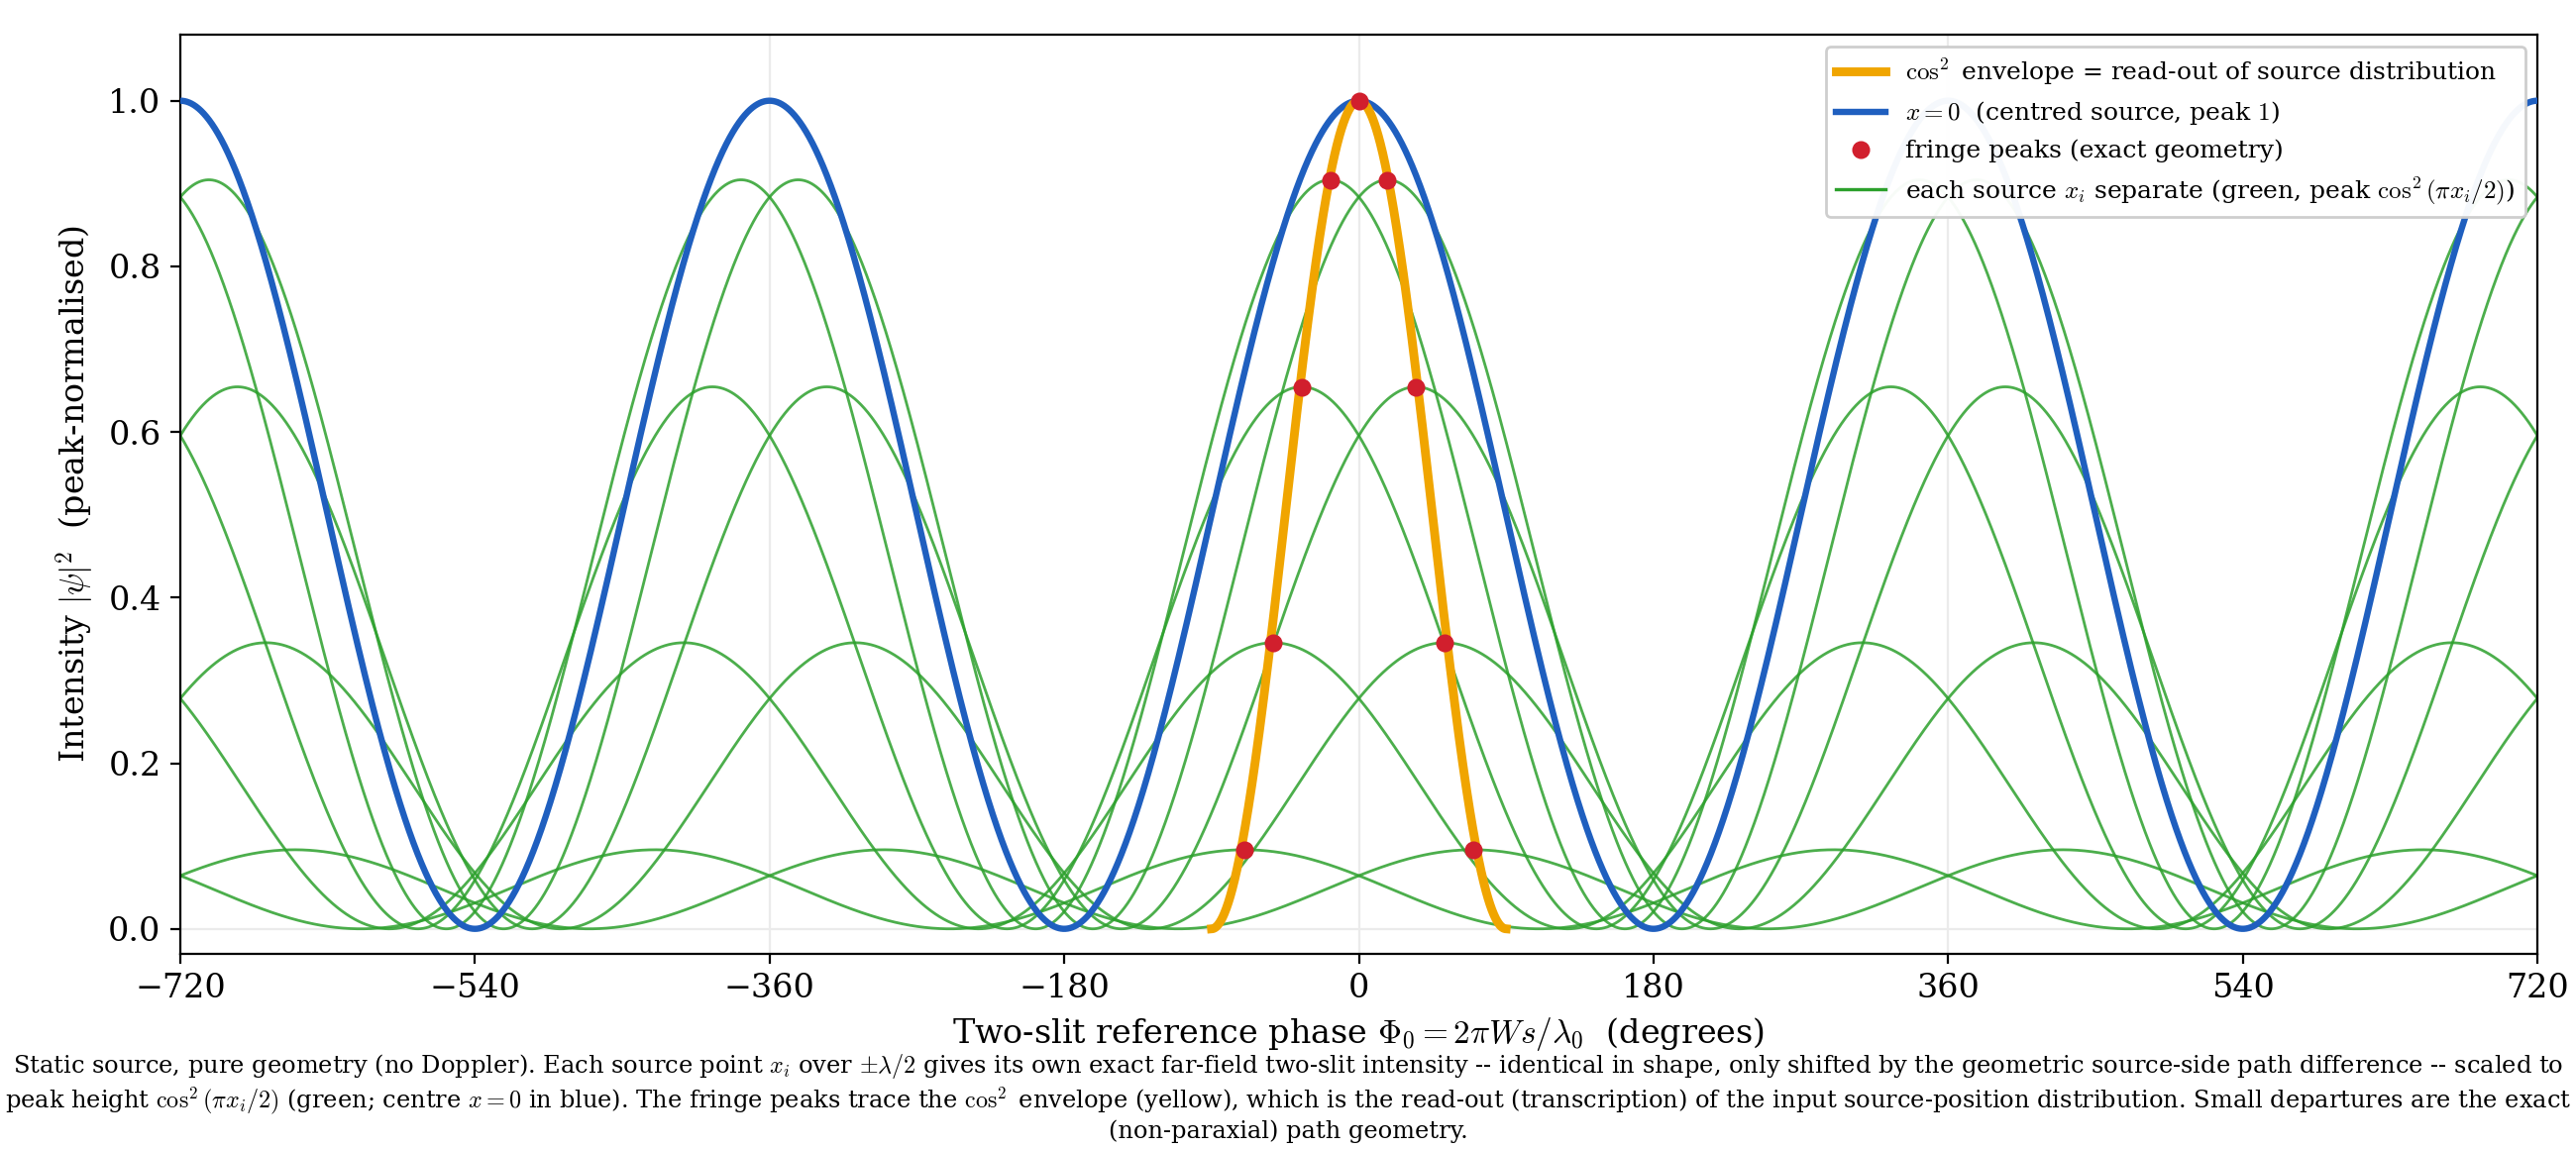
\includegraphics[keepaspectratio,alt={図3 各光源位置の縞（同形シフト）}]{fig_decomposition_static.png}}
\caption{図3 各光源位置の縞（同形シフト）}
\end{figure}

\emph{図3：静止光源・純幾何（ドップラー無し）。各光源位置 \(x\)
の厳密な遠方場二スリット強度は\textbf{同じ形で、光源側経路差だけシフト}する。各波形のピーク高さは重み
\(\cos^2(\pi x/2)\)（緑、中央 \(x=0\) は青）。各波形の縞ピーク（赤点）が
\(\cos^2\) 曲線（黄）をなぞる。}

これを反復試行のモンテカルロで直接確かめる。光源位置 \(y\) を \(P(y)\)
から引き、各試行で\textbf{縞シフト量 \(u(y)\)
だけを読んで}ヒストグラム化すると（図4）、\(\rho(u)\) は \(\cos^2\)
形を保つ。

\begin{figure}
\centering
\pandocbounded{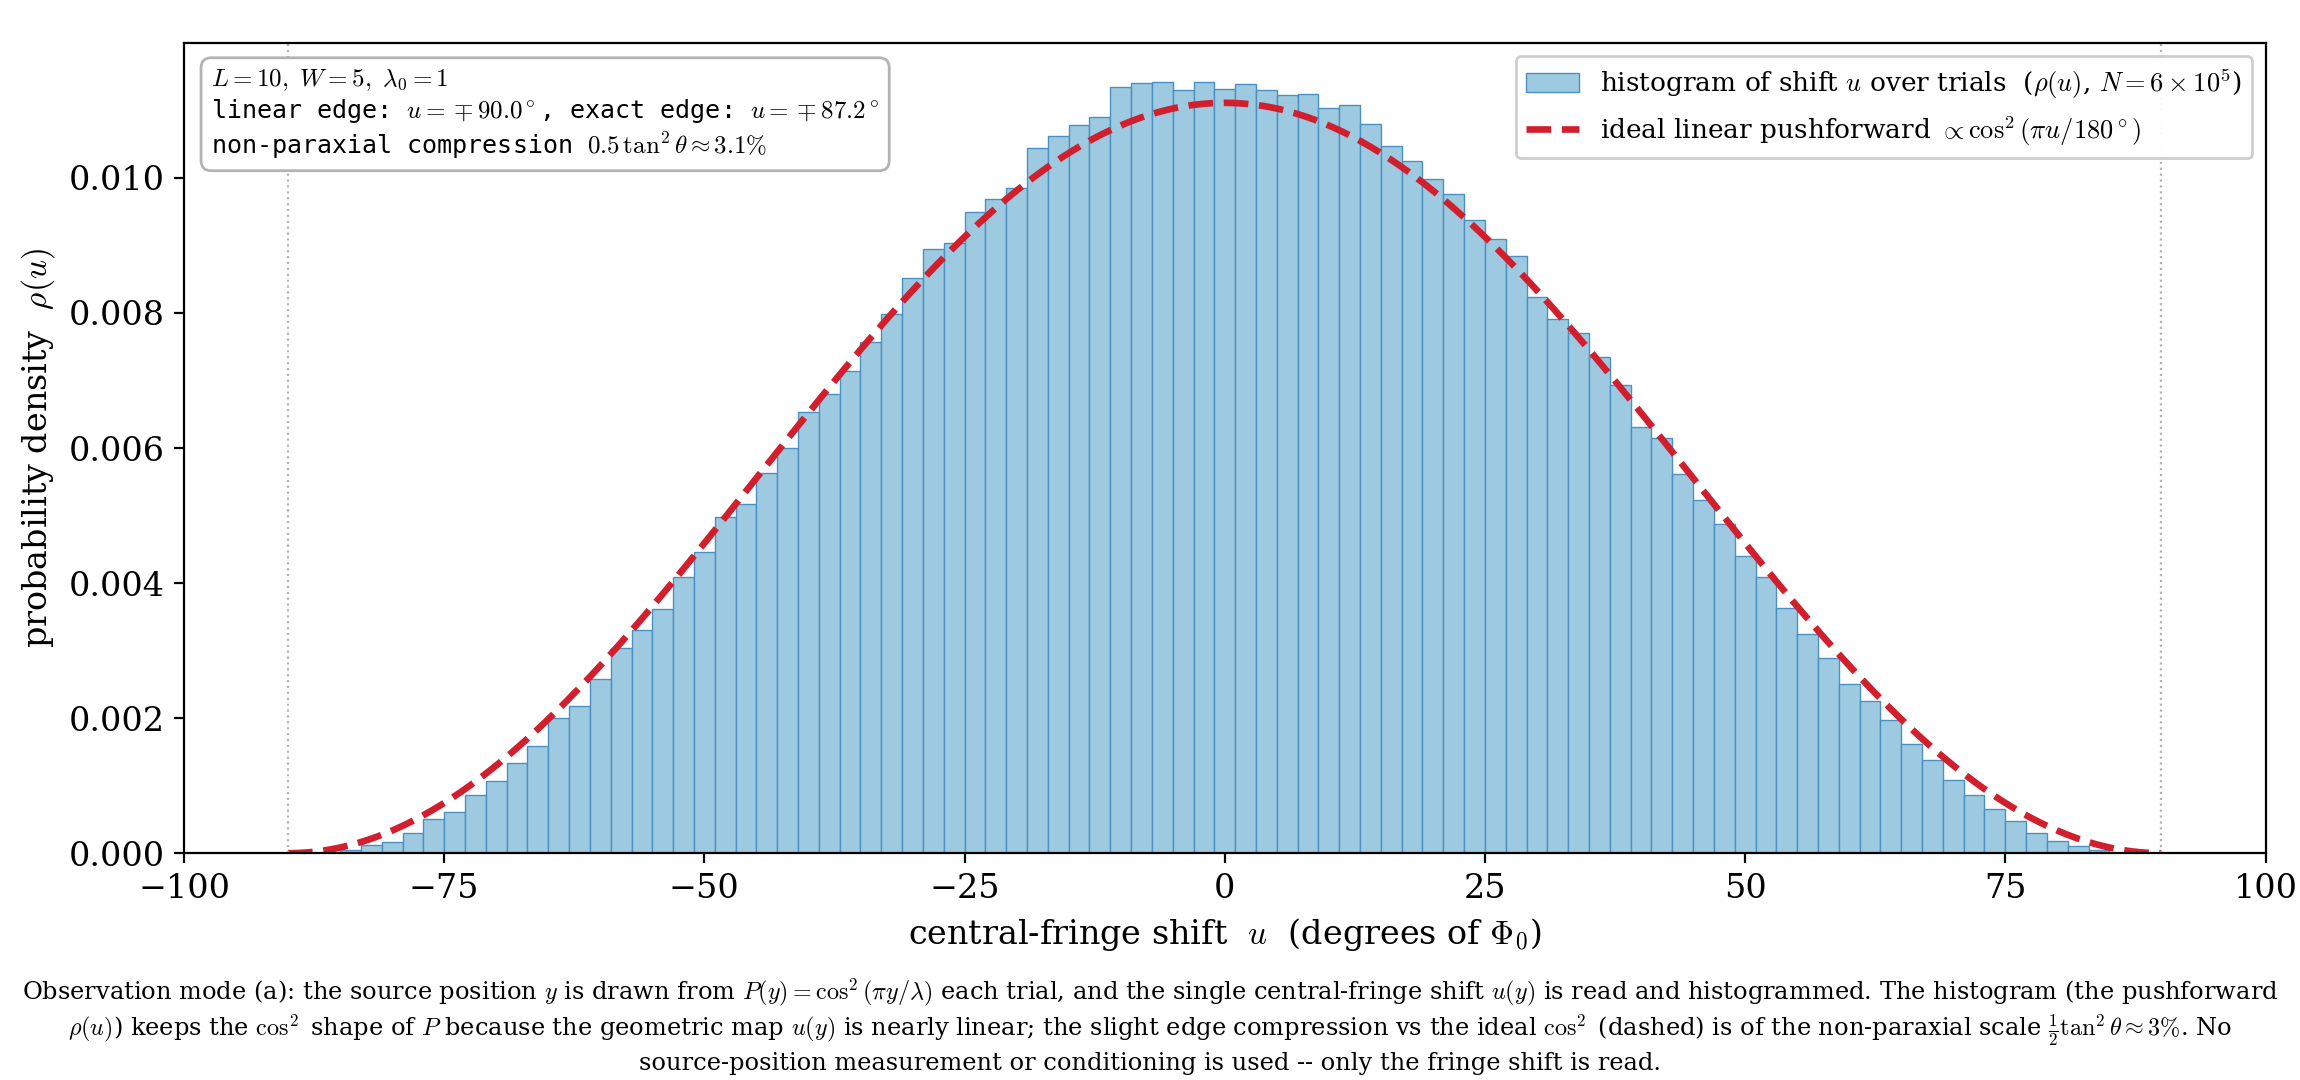
\includegraphics[keepaspectratio,alt={図4 シフト量のヒストグラム（押し出し）}]{fig_shift_histogram.png}}
\caption{図4 シフト量のヒストグラム（押し出し）}
\end{figure}

\emph{図4：観測モード(a)。各試行で \(y\sim P(y)\)
を引き、単一の縞シフト量 \(u(y)\)
を読んでヒストグラム化（\(N=6\times10^5\)）。ヒストグラム \(\rho(u)\) は
\(P\) の \(\cos^2\) 形を保つ（写像 \(u(y)\) がほぼ線形なため）。理想
\(\cos^2\)（赤破線）からの端の圧縮（厳密端 \(u=\mp87.2^\circ\) vs 線形
\(\mp90^\circ\)、\(3.09\%\)）が非近軸の非線形性（スケール
\(\tfrac12\tan^2\theta\approx3\%\)）。光源位置の測定も条件付けも用いず、縞シフトのみを読む。}

\subsubsection{4.2
一意性（エイリアシングの条件）}\label{ux4e00ux610fux6027ux30a8ux30a4ux30eaux30a2ux30b7ux30f3ux30b0ux306eux6761ux4ef6}

シフト量 \(u\) は中央（0次）縞の位置であり、本配置では
\(|u|\le u_{\max}=\dfrac{\pi W}{L}=90^\circ<180^\circ\)（縞周期
\(360^\circ\)
の半分）にとどまる。ゆえに0次縞は隣の次数（\(\pm360^\circ\)）と混ざらず、シフト量は一意に読める。\(W/L\)
や光源振れ幅が大きく \(u_{\max}\ge180^\circ\)
になると写像が巻き込み（エイリアス）、ヒストグラムが折り返す。本稿の押し出しが成り立つのはこの一意性の範囲内である。

\subsubsection{4.3 ずれの定量}\label{ux305aux308cux306eux5b9aux91cf}

\(\cos^2\) からのずれ（端で最大 \(\sim3\%\)）は、写像 \(u(y)\)
の非近軸非線形性に由来する。光源側経路差を展開すると、中心での傾き補正は
\(\tfrac12\tan^2\theta=\tfrac12(0.25)^2=3.13\%\)
である。一方モンテカルロの端圧縮は \(3.09\%\)
で、これは端で四次以降の項を含むため \(\tfrac12\tan^2\theta\)
と厳密には同一量ではないが、同じ非近軸スケール（\(\approx3\%\)）であり整合する。近軸極限
\(W/L\to0\) で \(u(y)\) は厳密に線形となり、形の保存は厳密になる。

\begin{center}\rule{0.5\linewidth}{0.5pt}\end{center}

\subsection{5. 考察}\label{ux8003ux5bdf}

\subsubsection{5.1 観測モードの明示 ―
何が押し出しになるのか}\label{ux89b3ux6e2cux30e2ux30fcux30c9ux306eux660eux793a-ux4f55ux304cux62bcux3057ux51faux3057ux306bux306aux308bux306eux304b}

本稿の分布は\textbf{単一の観測像の属性ではない}。区別すべき二つの観測モードがある。

\begin{itemize}
\tightlist
\item
  \textbf{(a)
  各試行で縞シフト量（中央ピーク位置）を読み、反復してヒストグラムを作る}
  → \(P\) の押し出し（図4）。これが本稿の主張である。光源位置 \(y\)
  を直接測る必要はなく、縞位置が \(y\)
  を符号化しているので、シフト量を読むだけでよい。
\item
  \textbf{(b) 多数試行の強度を一枚のスクリーンに積算する} →
  シフトで畳み込まれた\textbf{可視度の低下した単一縞}（\(2+2V\cos\),
  \(V<1\)）であって、入力分布の形にはならない。
\end{itemize}

一回の試行は一つのシフト量（一枚の縞）を与えるだけで、分布は現れない。形が現れるのは反復試行（アンサンブル）の統計としてである。これが成り立つには、\textbf{光源位置が1試行内で準静的（縞が立つ間は固定）で、試行間で揺らぐ}ことを要する（揺らぎが試行内で速いと
(b) になり消える）。得られるのは「分布を導出した」のではなく、入力
\(P(y)\) がシフト量分布へ写される\textbf{押し出し（変数変換）}である。

\subsubsection{5.2
慣性系について（限定的注記）}\label{ux6163ux6027ux7cfbux306bux3064ux3044ux3066ux9650ux5b9aux7684ux6ce8ux8a18}

同一の実験を任意の慣性系で（その系で静止させて）構成すれば、相対性原理により同じシフト量統計が得られる。これは相対性原理の自明な帰結であり、本稿はそれ以上を主張しない。とくに「検出事象の集合がローレンツ不変だから、一つの実験を動く観測者から見ても転写関係が成立する」という強い命題は\textbf{主張しない}（量的な縞間隔は光行差等で系に依存し、両辺の変換の整合は別途の計算を要する）。

\subsubsection{5.3
光源自体の並進は別問題（範囲外）}\label{ux5149ux6e90ux81eaux4f53ux306eux4e26ux9032ux306fux5225ux554fux984cux7bc4ux56f2ux5916}

本稿は放射点が動かない静止光源を扱う。光源自体が並進運動する設定（横速度
\(\beta_{\rm src}<1\)）は、二スリットが異なるドップラー振動数を受け、その振動数不一致に由来する可視度低下がシフト量の読み出しと競合する別問題であり、本稿の範囲外（今後の課題）とする。

\subsubsection{5.4 古典的描像（arcsine）との関係 ―
座標を明示する}\label{ux53e4ux5178ux7684ux63cfux50cfarcsineux3068ux306eux95a2ux4fc2-ux5ea7ux6a19ux3092ux660eux793aux3059ux308b}

光源を半径 \(\lambda/2\) の円周上を一様に巡る古典点 \(e^{i\theta}\)
とみなすとき、得られる分布は\textbf{どの座標で見るかに依存する}。

\begin{itemize}
\tightlist
\item
  \textbf{射影座標 \(x=\sin\theta\)}：一様な \(\theta\) の射影は逆正弦則
  \(p_A(x)=1/(\pi\sqrt{1-x^2})\)（端で発散の U
  字）。ここに振幅二乗の重み（Born 因子
  \(\cos^2\theta=1-x^2\)）を掛けると \(p\propto\sqrt{1-x^2}\)
  ＝\textbf{半円}であって \(\cos^2\) ではない。
\item
  \textbf{弧長座標 \(\theta\)（本稿の
  \(y\)、\(\theta=\pi y/\lambda\)）}：一様 → 一様。Born 因子
  \(\cos^2\theta\) を掛けると \(\cos^2\theta\)。本稿の \(P(y)\)
  はこちらである。
\end{itemize}

すなわち arcsine は射影座標 \(x\) に、\(\cos^2\) は弧長座標 \(\theta\)
に住んでおり、\textbf{同一座標の Born
因子では結ばれない}（座標の乗り換えが伴う）。なお Robinett (1995)
{[}1{]} は、調和振動子の古典確率密度が arcsine 型であり、量子
\(|\psi_n|^2\) が大 \(n\) 極限でこれに一致することを示す。これは
arcsine（射影座標・古典 HO の高 \(n\) 対応）の標準的裏づけであり、本稿の
\(\cos^2\)（弧長座標）と直接同一視するものではない。

\begin{center}\rule{0.5\linewidth}{0.5pt}\end{center}

\subsection{6. 結論}\label{ux7d50ux8ad6}

光源位置に揺らぎを持つ静止光源による二重スリット干渉について、純幾何の厳密計算により次を示した。

\begin{enumerate}
\def\labelenumi{\arabic{enumi}.}
\tightlist
\item
  一回の試行では、縞は\textbf{厳密に同形のまま} \(u(y)\)
  だけ左右にシフトする（波長一定、波形変形なし）。
\item
  光源位置 \(y\) を分布 \(P(y)\)
  から反復してランダムに引くと、\textbf{縞シフト量 \(u\) の確率分布は
  \(P\) の押し出しであり、写像 \(u(y)\) が近軸で線形ゆえ \(P\)
  の形が保存される}。これは \(\cos^2\)
  固有でなく線形写像の一般的帰結であり、本稿は \(P=\cos^2\) を例に同形の
  \(\cos^2\)
  が出ることを示した。形からのずれ（\(\sim3\%\)）は写像の非近軸非線形性（スケール
  \(\tfrac12\tan^2\theta\approx3\%\)）に由来し、近軸極限で消失する。シフト量は
  \(|u|<180^\circ\) の範囲で一意（エイリアスなし）。
\item
  この分布は\textbf{反復試行のシフト量統計}であって、単発の観測像でも、強度を積算した一枚像（可視度低下・形が崩れる）でもない。
\end{enumerate}

これは新しい確率法則の導出ではなく、入力分布が観測される統計量（縞シフト量）へ、近軸の線形幾何写像によって\textbf{形を保ったまま写される}ことの例示である。本稿は思考実験であり、確立した物理を例示・整理するものであって、それを覆すものではない。

\begin{center}\rule{0.5\linewidth}{0.5pt}\end{center}

\subsection{参考文献}\label{ux53c2ux8003ux6587ux732e}

{[}1{]} R. W. Robinett, ``Quantum and classical probability
distributions for position and momentum,'' \emph{American Journal of
Physics} \textbf{63}(9), 823--832 (1995). DOI: 10.1119/1.17807.

{[}2{]} M. Born and E. Wolf, \emph{Principles of Optics}, 7th (expanded)
ed.~(Cambridge University Press, 1999).

\begin{center}\rule{0.5\linewidth}{0.5pt}\end{center}

\emph{（再現コード：\texttt{fig\_setup\_double\_slit.py},
\texttt{fig\_setup\_source\_uncertainty.py},
\texttt{fig\_decomposition\_static.py},
\texttt{fig\_shift\_histogram.py}。\(\theta\)・経路はすべて \(L,W\)
から導出し、定数を恣意的に置いていない。移動仮定・ドップラーは用いない。）}

\end{document}
